\documentclass[12pt,notitlepage]{article}

%\usepackage{listings}
\usepackage[utf8]{inputenc}%jsta
\usepackage[english]{babel}%test
\usepackage{float}

\usepackage{natbib}
\usepackage[obeyspaces,spaces]{url}
\bibliographystyle{plainnat}
\bibpunct[; ]{(}{)}{,}{a}{}{;}

\usepackage{pifont,mdframed}%test

\usepackage{geometry}
\geometry{left=1.25in,right=1.25in,top=1.25in,bottom=1.25in}
\usepackage{rotating}
\usepackage{fancyhdr}
\usepackage[bookmarks,colorlinks,breaklinks,citecolor=red]{hyperref}
\usepackage{longtable}


%\usepackage{float}
\usepackage{graphicx,subfig}
% \usepackage{placeins}
\setlength\headheight{26pt}

\fancypagestyle{plain}{\fancyhf{}\fancyhead[R]{
\includegraphics[width=6.0in,keepaspectratio=true]{sfwmd_bar8half_wordorexcel.png}}}

\author{Joseph Stachelek}
\title{dbhydroR: An R package to access the DBHYDRO Environmental Database}

%\VignetteIndexEntry{An R package to access the DBHYDRO Environmental Database}

\usepackage{Sweave}
\begin{document}
\Sconcordance{concordance:dbhydroR.tex:dbhydroR.Rnw:%
1 34 1 1 0 14 1 1 4 11 1 1 2 4 0 1 2 7 1 1 2 %
4 0 1 2 3 1 1 3 5 0 1 2 2 1 1 3 5 0 1 2 2 1 %
1 3 5 0 1 2 2 1 1 4 6 0 1 2 4 1 1 4 6 0 1 2 %
6 1 1 2 4 0 1 2 3 1 1 2 4 0 1 2 2 1 1 2 1 0 %
2 1 3 0 1 2 2 1 1 2 4 0 1 2 5 1 1 2 4 0 1 2 %
2 1 1 3 5 0 1 2 1 1 1 3 5 0 1 2 2 1 1 3 5 0 %
1 2 6 1 1 2 4 0 1 2 3 1 1 4 3 0 1 2 3 0 1 2 %
2 1 1 3 2 0 1 1 3 0 1 2 53 1}

\maketitle
%\tableofcontents
 


\section{Introduction}

This document introduces the \texttt{dbhydroR} package and its associated functions. These functions are aimed at improving programmatic workflows that query the DBHYDRO Environmental Database. HTTP requests are faciliated by the httr \citep{httr} and RCurl \citep{rcurl} packages. 

\section{Package installation}

The \texttt{R} package \texttt{dbhydroR} is distributed via a \texttt{.tar.gz} (analagous to \texttt{.zip}) package archive file. This package contains the source code for package functions. In RStudio, it can be installed by navigating to \texttt{Tools} \verb|->| \texttt{Install Packages...} \verb|->| \texttt{Install from:} \verb|->| \texttt{Package Archive File}. Computers running the Windows operating system can only install binary \texttt{.zip} package archive files unless they have additional compiler software installed. The \texttt{dbhydroR} binary package can be installed by running the following command from the \texttt{R} console:

\vspace{10pt}
\noindent\texttt{install.packages(}\\
\path{"B:\\restoration_sciences\\projects\\joe_stachelek\\R\\dbhydroR_0.1-1.zip"}
\texttt{,type="win.binary",repos=NULL,dependencies=TRUE)}
\vspace{8pt}

Once installed, the package can be loaded using the following command:



\begin{Schunk}
\begin{Sinput}
> library(dbhydroR)
\end{Sinput}
\end{Schunk}



\section{Composing database queries}
\subsection{Water quality data}

The workhorse \texttt{dbhydroR} function is \verb|getwq| and \texttt{gethydro}. This function takes four required arguments. The user must specify a station ID, a test name, and a date range. Station IDs can be located on the \href{http://my.sfwmd.gov/KMLEXT/CUSTOMKMLS/DBHydro/DBHydroKML/DBHYDRO_KML.kmz}{SFWMD Google Earth portal}. A list of available test names can be found in the \nameref{sec:appendix} to this document. Dates must be specified in YYYY-MM-DD format (e.g. 2015-02-26).   The following set of examples retrieve measurements between March 2011 and May 2012. They can be run from the R console by issuing the command:

\begin{Schunk}
\begin{Sinput}
> example(getwq)
\end{Sinput}
\end{Schunk}

\begin{itemize}
\item One variable at one station

\begin{Schunk}
\begin{Sinput}
> getwq(station_id="FLAB08", date_min="2011-03-01",
+            date_max="2012-05-01",test_name="CHLOROPHYLLA-SALINE")
\end{Sinput}
\end{Schunk}

\item One variable at multiple stations

\begin{Schunk}
\begin{Sinput}
> getwq(station_id=c("FLAB08","FLAB09"), date_min="2011-03-01",
+            date_max="2012-05-01",test_name="CHLOROPHYLLA-SALINE")
\end{Sinput}
\end{Schunk}

\item One variable at a wildcard station

\begin{Schunk}
\begin{Sinput}
> getwq(station_id=c("FLAB0%"), date_min="2011-03-01",
+            date_max="2012-05-01",test_name="CHLOROPHYLLA-SALINE")
\end{Sinput}
\end{Schunk}

\item Multiple variables at multiple stations

\begin{Schunk}
\begin{Sinput}
> getwq(station_id=c("FLAB08","FLAB09"), date_min="2011-03-01",
+            date_max="2012-05-01",test_name=c("CHLOROPHYLLA-SALINE",
+                                              "SALINITY"))
\end{Sinput}
\end{Schunk}

\end{itemize}

\noindent By default, \verb|getwq| returns a "cleaned output". First, the cleaning function \verb|cleanwq| converts the raw output from native DBHYDRO "long" format (each piece of data on its own row) to "wide" format (each site x variable combination in its own column) using the reshape2 package \citep{reshape2}. Next, the QA blanks/flags and DBHydro database identifiers are stripped. Setting the \texttt{raw} flag to \texttt{TRUE} will force \verb|getwq| to retain this information. An example query that retains this information is shown below.

\begin{Schunk}
\begin{Sinput}
> getwq(station_id="FLAB08", date_min="2011-03-01",
+            date_max="2011-05-01",test_name="CHLOROPHYLLA-SALINE",
+            raw=TRUE)
\end{Sinput}
\end{Schunk}

\subsection{Hydrologic data}

Hydrologic time series data can be retrieved using the \texttt{gethydro} function. \texttt{gethydro} is a little more involved than \texttt{getwq} because there is no ability to perform wildcard matching and stations are identified not by name but by their "dbkey". The user must find the dbkey manually by navigating through the \href{http://my.sfwmd.gov/dbhydroplsql/show_dbkey_info.main_menu}{DBHYDRO Browser}. In addition to a dbkey, users must specify a date range. Dates must be entered in YYYY-MM-DD format (e.g. 2015-02-26).   The following set of examples retrieve wind speed measurements between January and February 2013. They can be run from the R console by issuing the command:

\begin{Schunk}
\begin{Sinput}
> example(gethydro)
\end{Sinput}
\end{Schunk}

\begin{itemize}
\item One variable/station time series
\begin{Schunk}
\begin{Sinput}
> gethydro(dbkey="15081",
+         date_min="2013-01-01",date_max="2013-02-02")
\end{Sinput}
\end{Schunk}

\item Multiple variable/station time series
\begin{Schunk}
\begin{Sinput}
> gethydro(dbkey=c("15081","15069"),
+         date_min="2013-01-01",date_max="2013-02-02")
\end{Sinput}
\end{Schunk}

\end{itemize}

\section{Plotting}

Once data has been retrieved with \verb|getwq| or \texttt{gethydro} in non-raw form (or raw water quality data that has been cleaned with \verb|cleanwq|), and assigned to an R object, plots can be produced using the \verb|dbhydro_plot| function. This function will create a dedicated panel of figures for each of the available variables. The following set of examples can be run from the R console by issuing the command:

\begin{Schunk}
\begin{Sinput}
> example(dbhydro_plot)
\end{Sinput}
\end{Schunk}

\begin{itemize}

\item{Water quality}
\begin{Schunk}
\begin{Sinput}
> dt<-getwq(station_id=c("FLAB08","FLAB09"),
+                date_min="2011-03-01",date_max="2014-05-01",
+                test_name=c("CHLOROPHYLLA-SALINE","SALINITY"))
> dbhydro_plot(dt,label="bottomleft",abb=3)
\end{Sinput}
\end{Schunk}


\item{Hydrologic}
\begin{Schunk}
\begin{Sinput}
> dt<-gethydro(dbkey=c("15081","15069"),
+             date_min="2013-01-01",date_max="2013-02-02")
> dbhydro_plot(dt)
\end{Sinput}
\end{Schunk}
\end{itemize}

\vspace{2pt}
\begin{figure}[H]
\begin{center}
%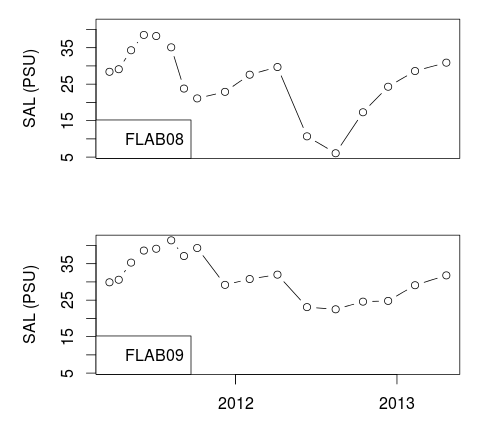
\includegraphics[width=12cm,height=10cm]{Rplot}
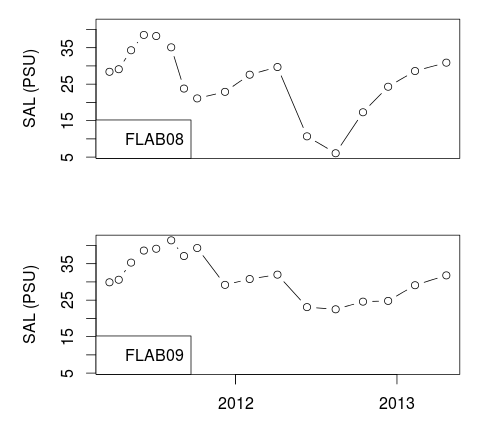
\includegraphics[width=343.5pt,height=310.8pt]{Rplot}
\end{center}
\label{fig:zero}
\end{figure}
%\FloatBarrier



\section{\label{sec:appendix}Appendix}
\subsection{Test names}
There are many test names available in DBHYDRO. These are detailed in the following table.\\

\begin{longtable}{| p{.45\textwidth} | p{.55\textwidth} |} 
\hline
Code\\
\hline
AMMONIA-N\\
CARBON, TOTAL ORGANIC\\
CHLOROPHYLL-A(LC)\\
CHLOROPHYLL-B(LC)\\
CHLOROPHYLLA-SALINE\\
DISSOLVED OXYGEN\\
KJELDAHL NITROGEN,TOTAL\\
NITRATE+NITRITE-N\\
NITRITE-N\\
PHEOPHYTIN-A(LC)\\
PHOSPHATE,ORTHO AS P\\
PHOSPHATE,TOTAL AS P\\
SALINITY\\
SILICA\\
SP CONDUCTIVITY, FIELD\\
TEMP\\
TOTAL NITROGEN\\
TURBIDITY\\
\hline
\end{longtable}
%\end{tabular}

\subsection{Further reading}
See section on URL-based data access in the \href{http://www.sfwmd.gov/portal/page/portal/xrepository/sfwmd_repository_pdf/dbhydrobrowseruserdocumentation.pdf}{DBHYDRO Browser User's Guide}

\medskip
 
 %\setlength{\bibsep}{0pt}
\bibliography{bib}

 
\end{document}
